Recent experiments have been collecting a significant amount of data.
Machine learning has become a very useful tool when processing this data.
A neural network is one section of machine learning that is heavily based off the structure of animal brains.
Where an animal brain is able to learn by activating specific neurons for thoughts and actions, the neurons in a machine learn in a similar vein through various kernels and learnable parameters.
These sets of neurons are divided into layers and generally show up as an input layer, some amount of hidden layers, and an output layer.
For our problem, the input layer will be the signal seen by the photomultiplier tubes in the top array of the detector, and the output layer will be the $(x,y)$ position of the interaction.
We are mainly concerned with graph convolutional neural networks (GCNNs) which are a result of the success with convolutional neural networks (CNNs).
\begin{figure}[t]
	\centering
	\begin{subfigure}{0.32\textwidth}
		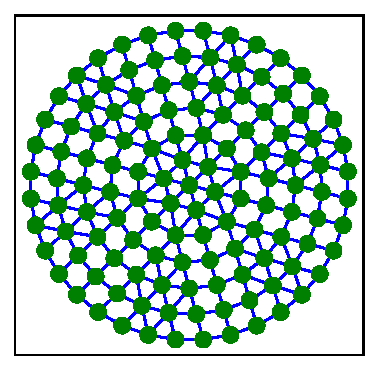
\includegraphics[width=\textwidth]{figures/1T_radius-graph_R10.pdf}
		\caption{}
	\end{subfigure}
	\begin{subfigure}{0.32\textwidth}
		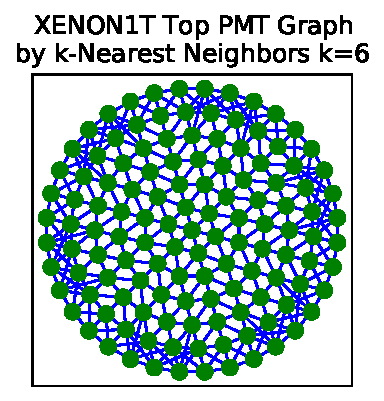
\includegraphics[width=\textwidth]{figures/1T_kNN-graph_k6.pdf}
		\caption{}
	\end{subfigure}
	\begin{subfigure}{0.32\textwidth}
		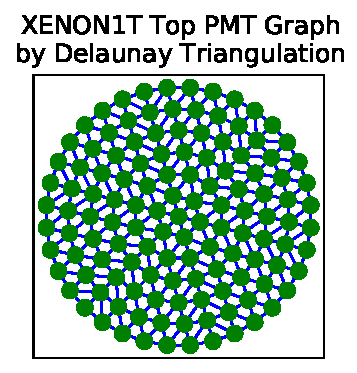
\includegraphics[width=\textwidth]{figures/1T_delaunay-graph.pdf}
		\caption{}
	\end{subfigure}
	\caption{
	Three of the considered graph structures: Radius $R=10$ cm neighbors (a), $k$-nearest-neighbors $k=6$ (b), Delaunay triangulation neighbors (c).
	Each node here is a photomultiplier tube in the top array of the XENON1T detector.
	The positions of each tube in the detector was used for each of the explored graph structure approaches.
	}
	\label{fig:graph_structs}
\end{figure}
\subsection{Convolutional Neural Networks}
A convolutional neural network is a specific kind of neural network that features a convolution layer.
The input to a CNN typically comes in the form of a matrix where there is a locality between the elements in the matrix.
The convolution layer makes use of a kernel that takes information from submatrices of the input matrix and summarizes the values within these submatrices.
These summaries maintain the locality of the information for the respective submatrices.
However, the structure of our dataset does not have a form that can be easily made into a matrix.
Therefore, we would need an algorithm that is capable of making use of datasets with any possible structure.
\begin{figure}[t]
	\centering
	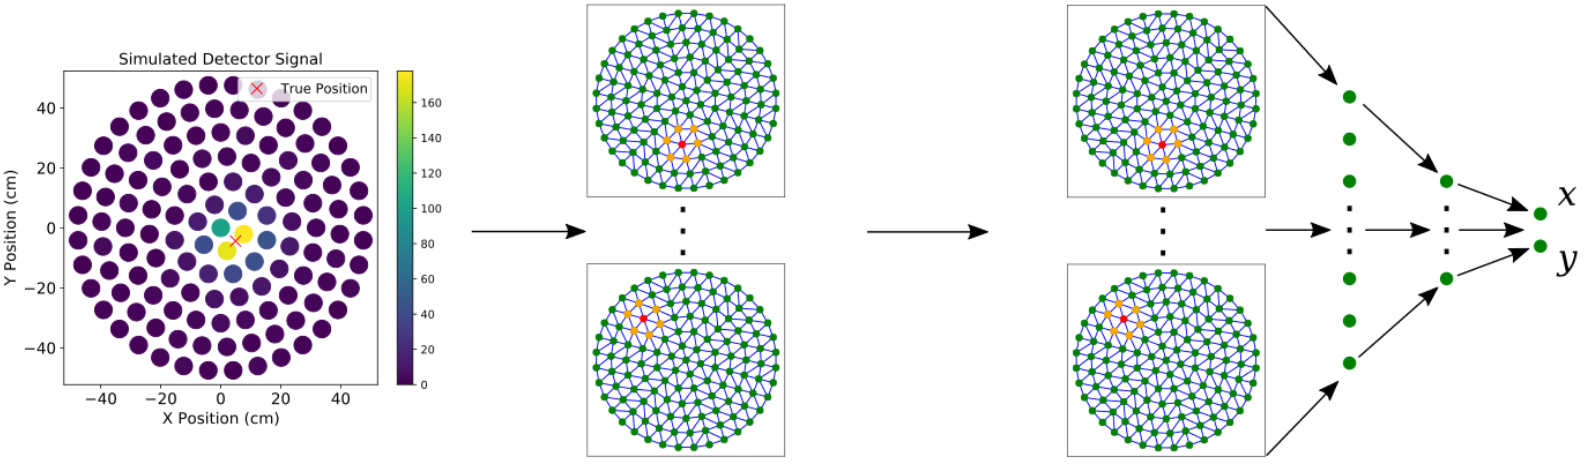
\includegraphics[width=\linewidth]{figures/GCNN_Structure.png}
	\caption{
	The graph convolutional neural network structure that the results of this paper are based on.
	The final structure features the signal input layer, two propagation (graph convolution) layers, two fully connected layers, and a final output layer for the $(x,y)$ position of the interaction.
	Between each layer is a ReLU activation function.
	There are a total of 57,486 trainable parameters.
	\\ TODO: Replace the image with a sharper PDF version with less white space between the first propagation layer and the second.
	}
	\label{fig:figures/GCNN_Structure}
\end{figure}
\subsection{Graph Convolutional Neural Networks}
The design of the graph convolutional neural network (GCNN) came by considering how a convolution could be applied to a graph structured dataset \cite{GCNN_Kipf}.
The graph convolution layer that we use and that was proposed by Kipf and Welling propagates the values of nodes according to the edges \cite{GCNN_Kipf}.
The value of connected nodes will increase according to the values of the connected nodes while nodes that are disconnected will see no change.
The exact propagation rule is given by the equation:
\begin{linenomath}\begin{equation}\label{eq:conv}
H^{(l+1)} = \sigma\left( \tilde{D}^{-1/2} \tilde{A} \tilde{D}^{-1/2} H^{(l)} W^{(l)} \right)
\end{equation}\end{linenomath}
where $H^{(0)}$ will be our initial input signal, $\tilde{A}$ and $\tilde{D}$ are respectively modified, unweighted adjacency and modified degree matrices, $W^{(l)}$ is the trainable weights matrix for the $l$\textsuperscript{th} layer, and $\sigma(\cdot)$ is an activation function \cite{GCNN_Kipf}.
The modified adjacency and degree matrices are to include self-loops.
This means that nodes will connect to themselves and propagate values to themselves when passed through the graph convolution layers.
The modified adjacency and degree matrices take the form:
\begin{linenomath}\begin{align*}
	\tilde{A} &= A + I_{N} \\
	\tilde{D} &= D + I_{N}
\end{align*}\end{linenomath}
where $I_{N}$ is a $N \times N$ identity matrix where $N$ is the number of nodes.

\par We considered the PMTs of the XENON1T detector as our nodes and their quantity of light collected as their primary value.
We also included the $(x,y)$ position of the PMT at the top of the detector as addition values.
When translating to equation (\ref{eq:conv}), the matrices take the form:
\begin{linenomath}\begin{align*}
	\tilde{A}, \tilde{D} \in \mathbb{R}^{127 \times 127} \\
	H^{(0)} \in \mathbb{R}^{127 \times 3} \\
	H^{(1)}, W^{(0)} \in \mathbb{R}^{127 \times w}
\end{align*}\end{linenomath}
where $w$ will depend on our choice of network structure.
We chose to use rectified linear units (ReLU) as our activation function for all layers.

\par With regard to the network structure, we were influenced by the success of image classifiers, such as AlexNet.
However, convolutional neural networks of this structure and graph convolutional neural networks in general are more often used for classification, while we have a regression problem.
Our reasoning to use a GCNN for predicting the position of interactions came from being able to encode the local structure of the XENON1T detector into the dataset.
By treating the nodes of our graph as the PMTs at the top of the detector, we understood that the connections or edges that we put in place would maintain the local structure if done carefully.
We considered several graph structures shown in Figure \ref{fig:graph_structs}.
We ultimately chose the Delaunay Triangulated graph for it's consistent connection density throughout the graph: only PMTs that are immediately near each other are connected and resulted in most nodes having 6 edges.
Only nodes that represent PMTs near the wall of the detector had degrees less than 6.
There is potential for finding the graph structure that describes the detector's data best, but for this we chose to go with a heuristic approach.
